% Ubah judul dan label berikut sesuai dengan yang diinginkan.
\section{Result and Discussion}
\label{sec:resultanddiscussion}

% Ubah paragraf-paragraf pada bagian ini sesuai dengan yang diinginkan.
\subsection{Pengujian Performa Model dengan menggunakan Variasi Jarak}

Pada skenario pengujian selanjutnya, model diuji berdasarkan beberapa variasi jarak. Pengujian jarak berguna untuk mengetahui performa dan tingkat akurasi model jika input citra diambil dari jarak yang berbeda-beda. Hal ini perlu diuji karena semakin jauh jarak pendeteksi citra, maka semakin kecil data visual citra yang diperoleh. Hasil validasi jarak yang digunakan adalah 30 sentimeter yang dapat dilihat pada Tabel \ref{tb:30cm}, 50 sentimeter pada Tabel \ref{tb:50cm}, 70 sentimeter pada Tabel \ref{tb:70cm}, dan 90 sentimeter pada Tabel \ref{tb:90cm}. Untuk contoh dataset variasi pengujian jarak dapat dilihat pada Gambar \ref{fig:Variasi Jarak Kamera}.

\begin{figure}[H]
  \centering
  \subfloat[30 sentimeter]{
    
\includegraphics[width=0.2\textwidth]{gambar/bab4/30.jpg}
    %\caption{30 sentimeter}
    \label{fig:imagea}}
    \hfil 
  \subfloat[50 sentimeter]{
    
\includegraphics[width=0.2\textwidth]{gambar/bab4/50.jpg}
    %\caption{50 sentimeter}
    \label{fig:imageb}}

  \subfloat[70 sentimeter]{
    
\includegraphics[width=0.2\textwidth]{gambar/bab4/70.jpg}
    %\caption{70 sentimeter}
    \label{fig:imagec}}
    \hfil
  \subfloat[90 sentimeter]{
    
\includegraphics[width=0.2\textwidth]{gambar/bab4/90.jpg}
    %\caption{90 sentimeter}
    \label{fig:imaged}}

  \caption{Variasi Jarak Kamera}
  \label{fig:Variasi Jarak Kamera}
\end{figure}

\begin{table}[ht]
  \caption{Hasil Validasi Nilai Model dengan Jarak 30 cm}
  \label{tb:30cm}
  \centering
  \begin{tabular}{|l|c|c|c|c|}
  \hline
  \rowcolor[HTML]{C0C0C0} 
  \textbf{Kelas} & \textbf{Accuracy} & \textbf{Precision} & \textbf{Recall} & \textbf{F1-Score} \\ \hline
  Kanan    & 100\%            & 100\%             & 100\%           & 100\%            \\ \hline
  Kiri     & 100\%          & 100\%           & 100\%           & 100\%           \\ \hline
  Maju      & 100\%          & 100\%           & 100\%          & 100\%          \\ \hline
  Mundur     & 100\%            & 100\%             & 100\%           & 100\%            \\ \hline
  Stop  & 100\%            & 100\%             & 100\%           & 100\%            \\ \hline
  \end{tabular}
\end{table}

\begin{table}[ht]
  \caption{Hasil Validasi Nilai Model dengan Jarak 50 cm}
  \label{tb:50cm}
  \centering
  \begin{tabular}{|l|c|c|c|c|}
  \hline
  \rowcolor[HTML]{C0C0C0} 
  \textbf{Kelas} & \textbf{Accuracy} & \textbf{Precision} & \textbf{Recall} & \textbf{F1-Score} \\ \hline
  Kanan    & 100\%            & 100\%             & 100\%           & 100\%            \\ \hline
  Kiri     & 100\%          & 100\%           & 100\%           & 100\%           \\ \hline
  Maju      & 100\%          & 100\%           & 100\%          & 100\%          \\ \hline
  Mundur     & 100\%            & 100\%             & 100\%           & 100\%            \\ \hline
  Stop  & 100\%            & 100\%             & 100\%           & 100\%            \\ \hline
  \end{tabular}
\end{table}

\begin{table}[ht]
  \caption{Hasil Validasi Nilai Model dengan Jarak 70 cm}
  \label{tb:70cm}
  \centering
  \begin{tabular}{|l|c|c|c|c|}
  \hline
  \rowcolor[HTML]{C0C0C0} 
  \textbf{Kelas} & \textbf{Accuracy} & \textbf{Precision} & \textbf{Recall} & \textbf{F1-Score} \\ \hline
  Kanan    & 100\%            & 100\%             & 100\%           & 100\%            \\ \hline
  Kiri     & 100\%          & 100\%           & 100\%           & 100\%           \\ \hline
  Maju      & 99.50\%          & 100\%           & 97.50\%          & 98.73\%          \\ \hline
  Mundur     & 99.50\%            & 97.56\%             & 100\%           & 98.77\%            \\ \hline
  Stop  & 100\%            & 100\%             & 100\%           & 100\%            \\ \hline
  \end{tabular}
\end{table}

\begin{table}[H]
  \caption{Hasil Validasi Nilai Model dengan Jarak 90 cm}
  \label{tb:90cm}
  \centering
  \begin{tabular}{|l|c|c|c|c|}
  \hline
  \rowcolor[HTML]{C0C0C0} 
  \textbf{Kelas} & \textbf{Accuracy} & \textbf{Precision} & \textbf{Recall} & \textbf{F1-Score} \\ \hline
  Kanan    & 100\%            & 100\%             & 100\%           & 100\%            \\ \hline
  Kiri     & 100\%          & 100\%           & 100\%           & 100\%           \\ \hline
  Maju      & 96.67\%          & 94.64\%           & 88.33\%          & 91.38\%          \\ \hline
  Mundur     & 96.67\%            & 89.06\%             & 95\%           & 91.94\%            \\ \hline
  Stop  & 100\%            & 100\%             & 100\%           & 100\%            \\ \hline
  \end{tabular}
\end{table}
    
\subsection{Pengujian Performa Model dengan menggunakan Variasi Pencahayaan}

Pada sistem kontrol kursi roda berbasis \emph{gesture} mata, variasi pencahayaan memiliki pengaruh signifikan terhadap performa model deteksi. Tujuan dari pengujian ini adalah untuk mengevaluasi tingkat keberhasilan dan ketidakberhasilan model dalam mendeteksi gerakan mata pada tiga kondisi pencahayaan, seperti pencahayaan redup (35 Lux) yang dapat dilihat pada Tabel \ref{tb:lux35}, normal (77 Lux) pada Tabel \ref{tb:lux55}, dan terang (131 Lux) pada Tabel \ref{tb:lux131}. Untuk variasi pengujian pencahayaan dapat dilihat pada Gambar \ref{fig:Variasi Pencahayaan}.

\begin{figure}[H]
  \centering
  \subfloat[35 Lux]{
    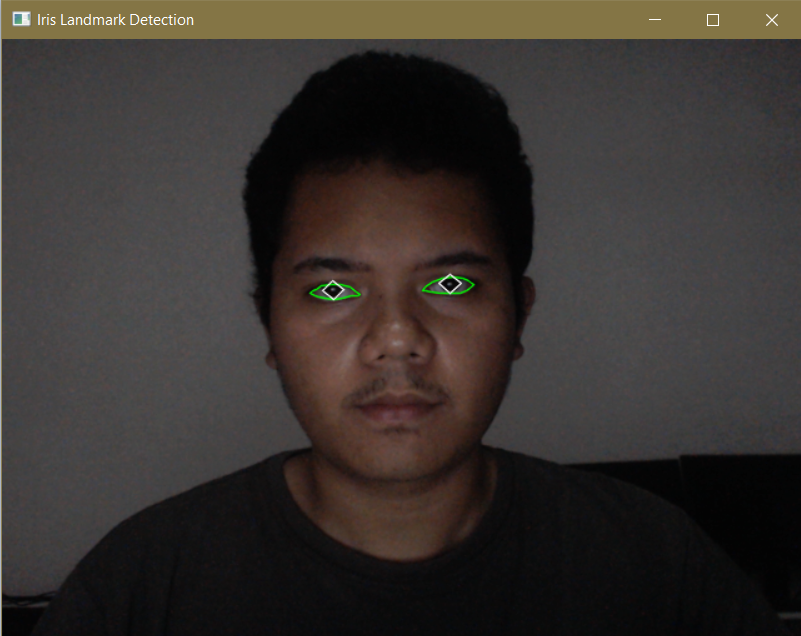
\includegraphics[width=0.15\textwidth]{gambar/bab4/33.png}
    %\caption{30 sentimeter}
    \label{fig:imageaa}}
  \hfil
  \subfloat[55 Lux]{
    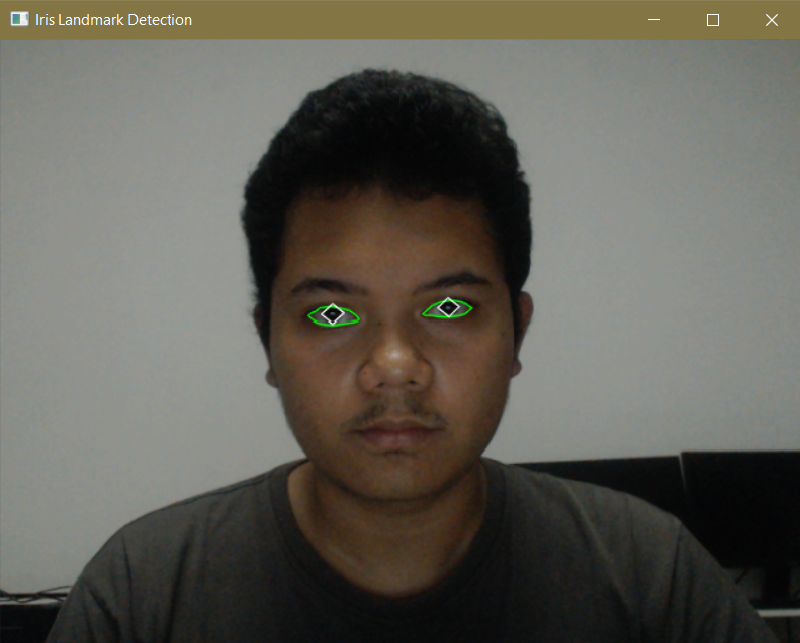
\includegraphics[width=0.15\textwidth]{gambar/bab4/55.png}
    %\caption{50 sentimeter}
    \label{fig:imagebb}}

  \subfloat[131 Lux]{
    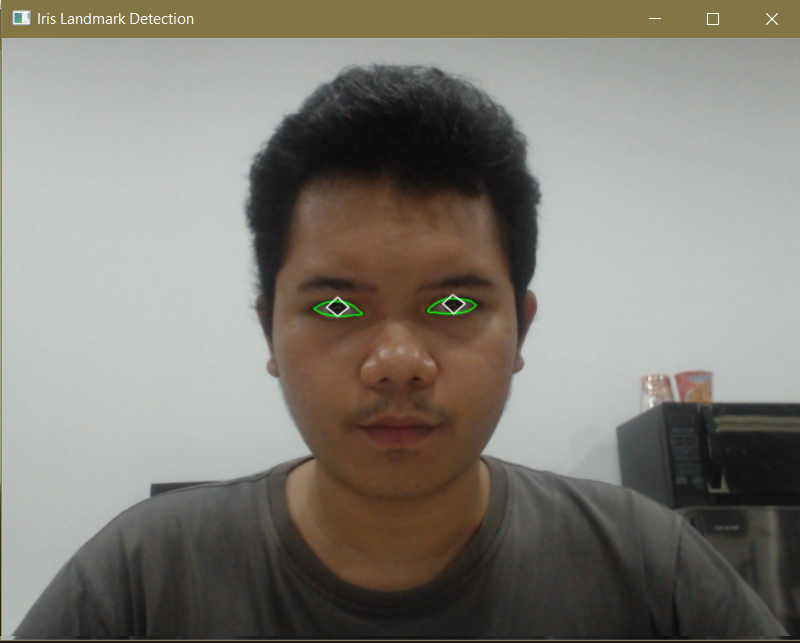
\includegraphics[width=0.15\textwidth]{gambar/bab4/131.png}
    %\caption{70 sentimeter}
    \label{fig:imagecc}}

  \caption{Variasi Pencahayaan}
  \label{fig:Variasi Pencahayaan}
\end{figure}

\begin{table}[ht]
  \caption{Pengujian Model dengan Pencahayaan 35 Lux}
  \label{tb:lux35} 
  \centering
  \begin{tabular}{|l|c|c|}
  \hline
  \rowcolor[HTML]{C0C0C0} 
  \textbf{Kelas} &  \multicolumn{1}{c|}{\textbf{\begin{tabular}[c]{@{}c@{}}Persentase \\ Keberhasilan\end{tabular}}} & \multicolumn{1}{c|}{\textbf{\begin{tabular}[c]{@{}c@{}}Persentase\\ Ketidakberhasilan\end{tabular}}} \\ \hline
  Kanan                                                                                                                                                                             & 100\%                                                                                   & 0\%                                                                                         \\ \hline
  Kiri                                                                                                                                                                               & 100\%                                                                                   & 0\%                                                                                         \\ \hline
  Maju                                                                                                                                                                              & 90\%                                                                                    & 10\%                                                                                        \\ \hline
  Mundur                                                                         & 93.33\%                                                                                 & 6.67\%                                                                                      \\ \hline
  Stop                                                                                          & 100\%                                                                                   & 0\%                                                                                         \\ \hline
\end{tabular}
\end{table}

\begin{table}[ht]
  \caption{Pengujian Model dengan Pencahayaan 55 Lux}
  \label{tb:lux55} 
  \centering
  \begin{tabular}{|l|c|c|}
  \hline
  \rowcolor[HTML]{C0C0C0} 
  \textbf{Kelas} &  \multicolumn{1}{c|}{\textbf{\begin{tabular}[c]{@{}c@{}}Persentase \\ Keberhasilan\end{tabular}}} & \multicolumn{1}{c|}{\textbf{\begin{tabular}[c]{@{}c@{}}Persentase\\ Ketidakberhasilan\end{tabular}}} \\ \hline
  Kanan                                                                                                                                                                             & 100\%                                                                                   & 0\%                                                                                         \\ \hline
  Kiri                                                                                                                                                                               & 100\%                                                                                   & 0\%                                                                                         \\ \hline
  Maju                                                                                                                                                                              & 96.67\%                                                                                    & 3.33\%                                                                                        \\ \hline
  Mundur                                                                         & 93.33\%                                                                                 & 6.67\%                                                                                      \\ \hline
  Stop                                                                                          & 100\%                                                                                   & 0\%                                                                                         \\ \hline
\end{tabular}
\end{table}

\begin{table}[H]
  \caption{Pengujian Model dengan Pencahayaan 131 Lux}
  \label{tb:lux131} 
  \centering
  \begin{tabular}{|l|c|c|}
  \hline
  \rowcolor[HTML]{C0C0C0} 
  \textbf{Kelas} &  \multicolumn{1}{c|}{\textbf{\begin{tabular}[c]{@{}c@{}}Persentase \\ Keberhasilan\end{tabular}}} & \multicolumn{1}{c|}{\textbf{\begin{tabular}[c]{@{}c@{}}Persentase\\ Ketidakberhasilan\end{tabular}}} \\ \hline
  Kanan                                                                                                                                                                             & 100\%                                                                                   & 0\%                                                                                         \\ \hline
  Kiri                                                                                                                                                                               & 100\%                                                                                   & 0\%                                                                                         \\ \hline
  Maju                                                                                                                                                                              & 100\%                                                                                    & 100\%                                                                                        \\ \hline
  Mundur                                                                         & 100\%                                                                                 & 100\%                                                                                      \\ \hline
  Stop                                                                                          & 100\%                                                                                   & 0\%                                                                                         \\ \hline
\end{tabular}
\end{table}

\subsection{Pengujian Performa \emph{Frame Per Second} (FPS) pada Sistem Kontrol Kursi Roda}

Pengujian performa \emph{Frame Per Second} (FPS) bertujuan untuk mengevaluasi kecepatan sistem dalam memproses gerakan mata secara real-time untuk mengontrol kursi roda. FPS merupakan indikator penting dalam menilai kelancaran dan responsivitas sistem, terutama dalam aplikasi yang memerlukan deteksi gerakan dan pengambilan keputusan yang cepat. Hasil pengujian FPS pada laptop dan NUC dapat dilihat pada Tabel \ref{tb:fps}.

\begin{table}[H]
  \caption{Hasil Performa FPS pada Laptop dan NUC}
  \label{tb:fps}
  \centering
  \begin{tabular}{|l|c|c|}
  \hline
  \rowcolor[HTML]{C0C0C0} 
  \textbf{Kelas} & \textbf{Rata-rata FPS Laptop} & \textbf{Rata-rata FPS NUC} \\ \hline
  Kanan           & 12.745              & 10.567           \\ \hline
  Kiri           & 12.635              & 10.617            \\ \hline
  Maju           & 13.078              & 10.068           \\ \hline
  Mundur           & 13.507              & 9.734           \\ \hline
  Stop           & 12.580              & 10.127            \\ \hline
  \end{tabular}
\end{table}

\subsection{Pengujian Waktu dari \emph{Inference Time} pada Model ke \emph{Response Time} pada Motor Kursi Roda}

Pengujian waktu dari \emph{Inference Time} pada model ke \emph{Response Time} pada motor kursi roda bertujuan untuk mengevaluasi seberapa cepat sistem kontrol kursi roda berbasis gerakan mata dapat merespons perintah dari pengguna. \emph{Inference Time} mengukur waktu yang dibutuhkan oleh model untuk mendeteksi dan mengklasifikasikan gerakan mata, sementara \emph{Response Time} mengukur waktu yang diperlukan motor kursi roda untuk mulai bergerak setelah menerima sinyal dari model. Hasil pengujian waktu dari \emph{Inference Time} dan \emph{Response Time} dapat dilihat pada Tabel \ref{tb:response}.

\begin{table}[H]
  \caption{Hasil Pengujian Inference Time dan Response Time}
  \label{tb:response}
  \centering
  \begin{tabular}{|l|c|c|}
  \hline
  \rowcolor[HTML]{C0C0C0} 
  \textbf{Kelas} &  \multicolumn{1}{c|}{\textbf{\begin{tabular}[c]{@{}c@{}}Rata-rata \\ Inference Time (s)\end{tabular}}} & \multicolumn{1}{c|}{\textbf{\begin{tabular}[c]{@{}c@{}}Rata-rata\\ Response Time\end{tabular}}} \\ \hline
  Kanan           & 0.0626             & 0.2328           \\ \hline
  Kiri           & 0.0640              & 0.0933            \\ \hline
  Maju           & 0.0656               & 0.4337           \\ \hline
  Mundur           & 0.0637              & 0.1409           \\ \hline
  Stop           & 0.0666              & 0.4318            \\ \hline
  \end{tabular}
\end{table}

\subsection{Pengujian Kestabilan pada Motor Kursi Roda}

Pengujian kestabilan pada motor kursi roda bertujuan untuk memastikan bahwa waktu output yang dijalankan oleh motor tetap stabil untuk setiap input yang diberikan oleh pengguna melalui sistem kontrol gerakan mata. Pengujian ini melibatkan pengukuran waktu yang dibutuhkan oleh motor untuk merespons setiap perintah gerakan mata dan memastikan bahwa waktu respons tersebut tetap konsisten di berbagai kondisi input. Hasil pengujian kestabilan motor dapat dilihat pada Tabel \ref{tb:stabil}.

\begin{table}[H]
  \caption{Hasil Pengujian Kestabilan Motor}
  \label{tb:stabil}
  \centering
  \begin{tabular}{|l|c|c|}
  \hline
  \rowcolor[HTML]{C0C0C0} 
  \textbf{Kelas} &  \multicolumn{1}{c|}{\textbf{\begin{tabular}[c]{@{}c@{}}Rata-rata \\ Lama Motor Berjalan (s)\end{tabular}}} \\ \hline
  Kanan          & 6.013                        \\ \hline
  Kiri           & 6.469                          \\ \hline
  Maju           & 6.532                         \\ \hline
  Mundur         & 6.863                         \\ \hline
  Stop           & 4.933                          \\ \hline
  \end{tabular}
\end{table}